% !TEX root = ../main.tex
\section{Experiments}

\subsection{Experimental Setup}

We evaluate the proposed system using the evaluation suite described in
Section~4. The three experimental settings examine three questions in sequence.
The first evaluates whether the complete framework can execute the end-to-end
decision loop across different downstream foundation-model configurations as
operational pressure increases. The second examines how Validation, Memory, and
Runtime Replanning address their respective decision risks under increasing
operational pressure. The third assesses whether validated decision traces can
specialize a lower-overhead compact planner for resource-constrained mission
planning. 

To isolate the influence of the foundation model on Mission Planning,
Validation, and Runtime Replanning, we fix Gemini~3.1~Pro as the foundation
model for Vision Analysis in the first setting. We then evaluate four
configurations by using ChatGPT~5.5, Gemini~3.1~Pro, Claude~Opus~4.7, and
DeepSeek~V4~Pro, respectively, in the remaining LLM-based modules. This design
keeps the transformation from aerial imagery to the structured fire situation
consistent across configurations, allowing their subsequent differences to
reflect the models used in Mission Planning, Semantic Validation, and Runtime
Replanning. The four configurations are controlled variants of the proposed
system rather than external algorithmic baselines; because Vision Analysis is
fixed, the comparison concerns the downstream decision modules. Each
configuration is evaluated on the same 80 episodes, comprising 20 episodes at
each of the simple, normal, hard, and expert difficulty levels.

For the second setting, we use the DeepSeek~V4~Pro configuration and compare the
full system with three ablated variants: w/o Validation, w/o Memory, and w/o
Runtime Replanning. The first removes the semantic and deterministic
audit--correction loop; the second disables retrieval from both Episodic Memory
and Lesson Memory; and the third retains the initial plan after runtime
perturbations without invoking Runtime Replanning. All other models, prompts,
and execution settings remain unchanged. All four configurations are evaluated
on the same 80 episodes, with 20 episodes at each difficulty level. In the
simple and normal settings, where no runtime perturbations occur, the w/o
Runtime Replanning variant differs only in that the Runtime Replanning module
is disabled and therefore remains inactive throughout execution.

For the third setting, we construct 2,000 mission-planning demonstrations
using the proposed system with Gemini~3.1~Pro as the teacher planner. The
demonstrations are generated from mission situations disjoint from the 80
evaluation episodes. Each demonstration has the form
\[
(R,U,C) \rightarrow P,
\]
where each demonstration pairs a structured description of the task zones, UAV
states, and mission constraints with the final multi-UAV plan accepted after the
Semantic Validation and Deterministic Rule Validation loop. We use these
validated demonstrations to specialize Qwen3-8B for the planning mapping
defined in Section~3. The dataset is divided into 90\% for training and 10\%
for validation. We apply 4-bit quantized low-rank adaptation with a maximum
sequence length of 6,144 tokens. The model is trained for three epochs with an
effective batch size of 16 and a learning rate of $5\times10^{-5}$. Fine-tuning
is conducted on a single NVIDIA GeForce RTX~4090, with 16 Intel Xeon Gold~6430
vCPUs and 120~GB of system memory.

We evaluate both the original and fine-tuned Qwen3-8B by replacing only the
planner used by Mission Planning. Vision Analysis and Semantic Validation
continue to use Gemini~3.1~Pro, while Deterministic Rule Validation and all
other non-LLM components remain unchanged. The two Qwen3-8B configurations are
evaluated on the same 40 simple and normal episodes used in the first setting,
with 20 episodes at each level. Because these levels contain no runtime perturbations,
this experiment does not invoke Runtime Replanning or assess event stability.
The comparison therefore isolates the effect of planner fine-tuning on the
same episode subset.

\subsection{End-to-End Evaluation}

Before examining individual mechanisms, we first evaluate the complete system
across multiple foundation-model configurations. This experiment establishes
end-to-end task performance under the proposed evaluation setting and examines
the sensitivity of the downstream decision process to model choice.
Its primary purpose is to determine whether the full decision loop can be
executed across the evaluated configurations, rather than to produce a
general ranking of foundation models.
Table~\ref{tab:main-results} reports the results across all four difficulty
levels, while Figure~\ref{fig:model-total-score} summarizes the overall scores.
All configurations achieve complete task coverage in the simple and
normal episodes, near-complete coverage in the hard episodes, and completion
scores above 90 in the expert episodes. Thus, each evaluated configuration can
support the full decision loop from the shared Vision Analysis output to
mission execution, although the quality and continuity of execution vary with
operational pressure.

\begin{figure}[!t]
    \centering
    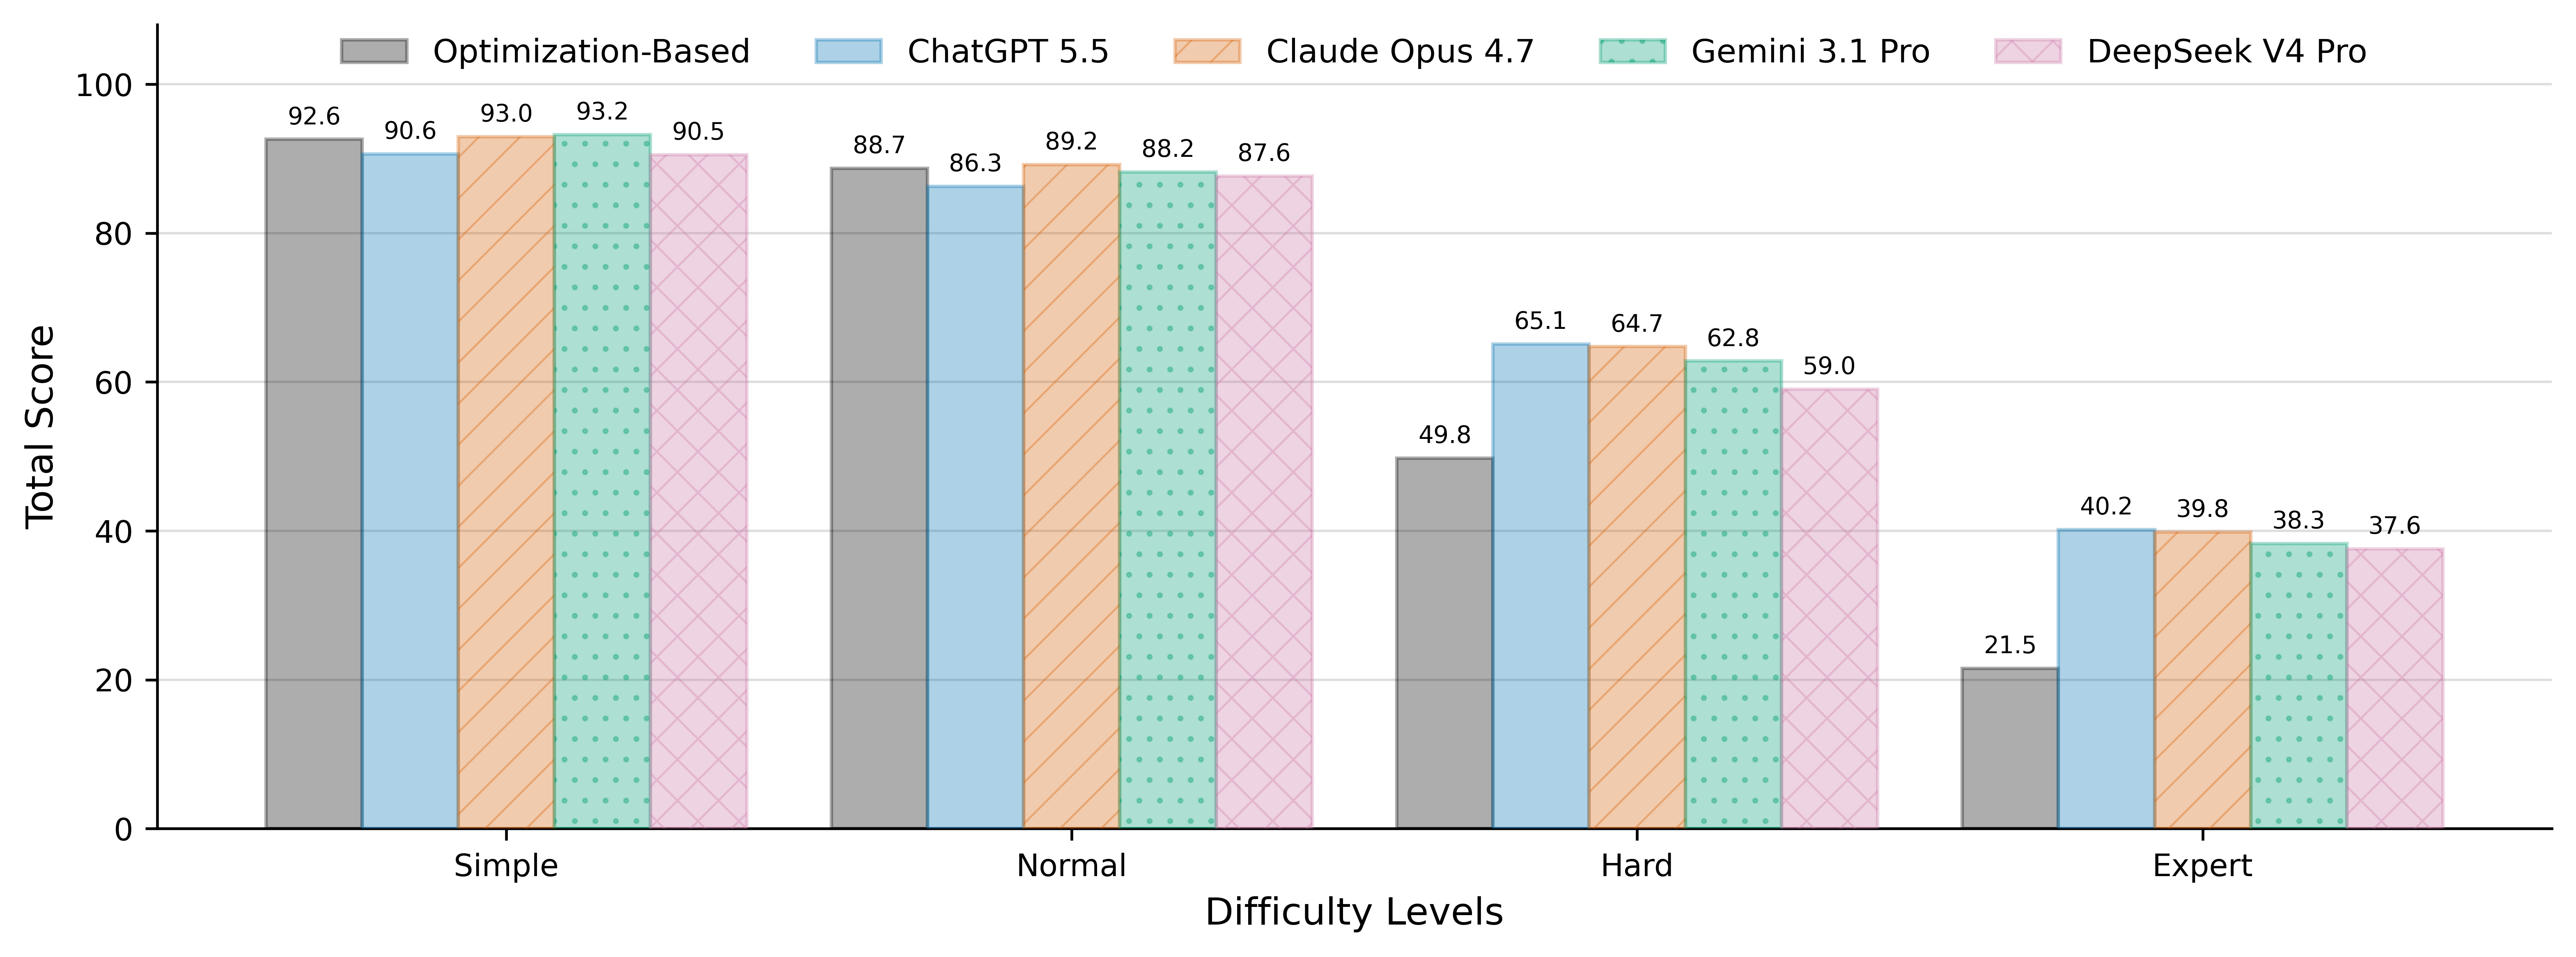
\includegraphics[width=\columnwidth]{figures/foundation-model-overall-scores.png}
    \caption{Overall scores of the four foundation-model configurations across
    episode difficulty levels.}
    \label{fig:model-total-score}
\end{figure}

\begin{table*}[!t]
    \centering
    \caption{End-to-end results for the Optimization-Based Planner and the
    proposed framework across episode difficulty levels. Optimization-Based
    denotes the Optimization-Based Planner, while each model name denotes the
    corresponding downstream foundation-model configuration of the proposed
    framework.
    $S$ is the overall score, and the remaining columns report normalized mission-level scores in
    $[0,100]$ (higher is better). Event stability is not applicable to the
    simple and normal settings and is denoted by ``--''. The highest observed
    value for each metric at every difficulty level is shown in bold when it is
    unique; these highlights describe the evaluated configurations rather than
    a general ranking of foundation models.}
    \label{tab:main-results}
    \footnotesize
    \setlength{\tabcolsep}{1.5pt}
    \renewcommand{\arraystretch}{1.12}
    \begin{tabular*}{\textwidth}{@{\extracolsep{\fill}}llcrrrrrr@{}}
        \toprule
        \multirow{2}{*}{\textbf{Difficulty}}
        & \multirow{2}{*}{\textbf{Configuration}}
        & \multirow{2}{*}{\textbf{$S$}}
        & \multicolumn{6}{c}{\textbf{Mission-level score}} \\
        \cmidrule(l){4-9}
        & &
        & \textbf{Completion}
        & \textbf{Response}
        & \textbf{Time}
        & \makecell{\textbf{Event}\\\textbf{stability}}
        & \makecell{\textbf{Resource}\\\textbf{pressure}}
        & \textbf{Coordination} \\
        \midrule

        Simple & Optimization-Based
        & 92.59 & 100.00 & \textbf{92.34} & 88.94
        & -- & \textbf{85.64} & 82.31 \\
        & ChatGPT~5.5
        & 90.63 & 100.00 & 89.18 & 78.99
        & -- & 81.20 & 79.54 \\
        & Gemini~3.1~Pro
        & \textbf{93.23} & 100.00 & 88.78 & \textbf{91.06} & -- & 84.45 & 80.71 \\
        & Claude~Opus~4.7
        & 92.97 & 100.00 & 91.44 & 86.62 & -- & 82.18 & \textbf{83.96} \\
        & DeepSeek~V4~Pro
        & 90.54 & 100.00 & 87.66 & 78.90 & -- & 83.05 & 80.04 \\
        \addlinespace

        Normal & Optimization-Based
        & 88.72 & 100.00 & 89.07 & \textbf{72.71}
        & -- & \textbf{87.05} & 77.74 \\
        & ChatGPT~5.5
        & 86.28 & 100.00 & 93.82 & 66.27
        & -- & 77.64 & 73.19 \\
        & Gemini~3.1~Pro
        & 88.23 & 100.00 & 94.10 & 71.50 & -- & 86.68 & 71.72 \\
        & Claude~Opus~4.7
        & \textbf{89.18} & 100.00 & \textbf{96.09} & 68.24 & -- & 84.54 & \textbf{78.12} \\
        & DeepSeek~V4~Pro
        & 87.63 & 100.00 & 91.36 & 71.74 & -- & 83.95 & 75.13 \\
        \addlinespace

        Hard & Optimization-Based
        & 49.77 & 96.40 & 78.32 & 26.94
        & 20.75 & 54.86 & 52.14 \\
        & ChatGPT~5.5
        & \textbf{65.09} & 100.00 & \textbf{94.97} & \textbf{41.22}
        & \textbf{42.25} & \textbf{63.19} & \textbf{67.24} \\
        & Gemini~3.1~Pro
        & 62.81 & 100.00 & 92.58 & 39.60 & 33.75 & 59.10 & 60.65 \\
        & Claude~Opus~4.7
        & 64.74 & 99.86 & 94.22 & 35.28 & 40.50 & 62.15 & 65.88 \\
        & DeepSeek~V4~Pro
        & 59.03 & 98.57 & 83.90 & 30.76 & 34.75 & 61.36 & 59.07 \\
        \addlinespace

        Expert & Optimization-Based
        & 21.53 & 78.27 & 42.13 & 1.93
        & 0.00 & 42.07 & 39.87 \\
        & ChatGPT~5.5
        & \textbf{40.15} & \textbf{93.24} & \textbf{67.01} & \textbf{13.23}
        & \textbf{2.67} & \textbf{60.15} & \textbf{61.25} \\
        & Gemini~3.1~Pro
        & 38.28 & 90.09 & 61.30 & 12.02 & 0.00 & 58.72 & 55.82 \\
        & Claude~Opus~4.7
        & 39.81 & 92.43 & 65.55 & 9.13 & 0.00 & 58.99 & 60.11 \\
        & DeepSeek~V4~Pro
        & 37.55 & 90.95 & 61.09 & 3.54 & 0.00 & 53.43 & 54.43 \\
        \bottomrule
    \end{tabular*}
\end{table*}


The overall scores are closely grouped in the simple setting
(90.54--93.23) and the normal setting (86.28--89.18). The spread increases in
the hard setting (59.03--65.09) and narrows again once every configuration
encounters the severe expert-level conditions (37.55--40.15). The highest
observed score is obtained by Gemini~3.1~Pro in simple episodes,
Claude~Opus~4.7 in normal episodes, and ChatGPT~5.5 in hard and expert episodes.
Because this ordering changes with difficulty, the results do not yield a
single model ranking. Instead, the differences arise primarily in execution
quality: response, mission time, resource pressure, coordination, and recovery
from runtime events become more discriminative as operational pressure
increases.

Figure~\ref{fig:model-performance-radar} further compares the six
mission-level metrics. In the simple and normal settings, the model profiles
largely overlap near the outer region of the plots, although differences in
time efficiency and coordination are already visible. As operational pressure
increases, the profiles contract and differences become clearer in mission
time, coordination, resource pressure, and event stability. The resulting
variation shows that model choice affects how the downstream modules manage
execution under higher operational pressure, even though task completion
remains similar across configurations.

\begin{figure}[!htbp]
    \centering
    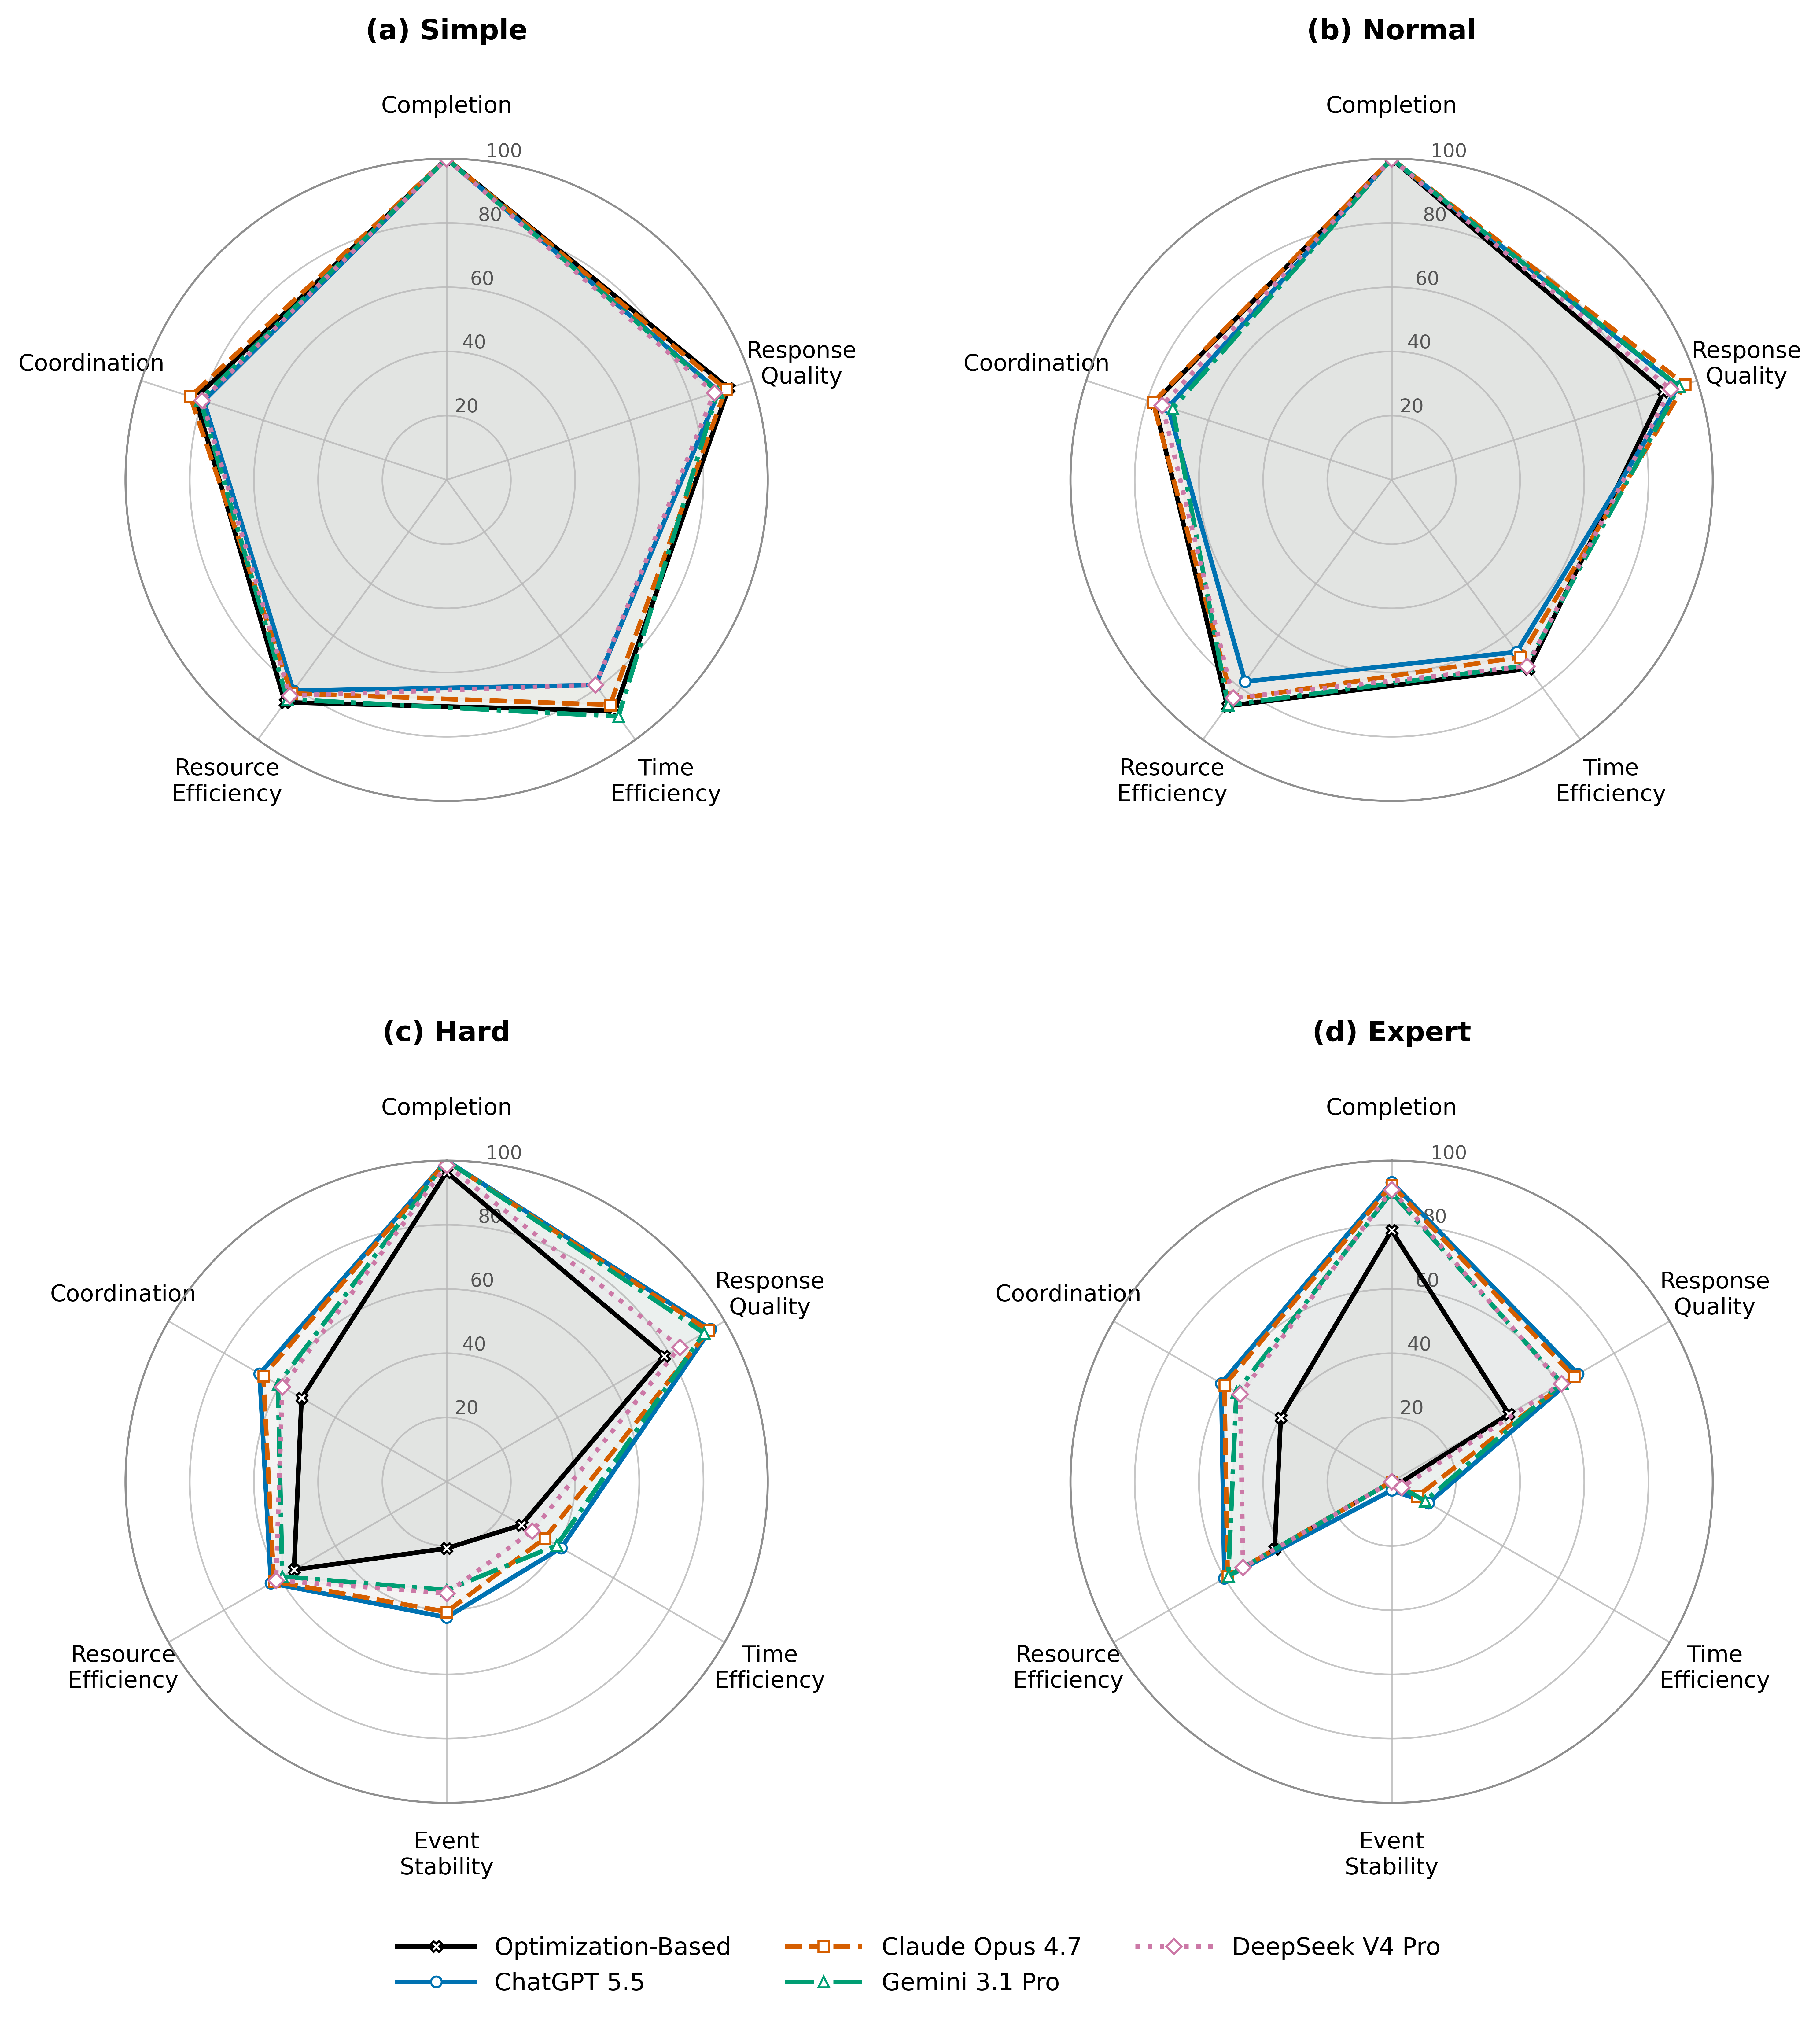
\includegraphics[width=0.95\columnwidth]{figures/foundation-model-performance-radar.png}
    \caption{Mission-level performance profiles of the four foundation-model
    configurations at each difficulty level. Larger radial values indicate
    better performance.}
    \label{fig:model-performance-radar}
\end{figure}

Increasing operational pressure across the difficulty levels nevertheless
degrades every configuration.
The most pronounced changes occur in mission time and event stability: time
scores fall to 3.54--13.23 in expert episodes, while event-stability scores
fall to 0--2.67. By contrast, expert-level completion remains above 90 for all
models. Thus, the principal challenge in the hardest episodes is not whether
the system can eventually complete the rescue tasks, but whether it can do
so efficiently while preserving mission continuity under repeated runtime
perturbations. Changing the foundation model alone does not prevent this common
degradation, exposing clear headroom for more robust replanning and time-aware
resource allocation. Taken together, the results show that the complete
decision loop maintains high basic task completion across the evaluated
downstream models, rather than depending on a single downstream foundation
model. At the same time, the common decline in execution quality and mission
continuity establishes the operational-pressure regime in which the roles of
the closed-loop mechanisms must be examined.

\subsection{Ablation Studies}

Having established the end-to-end behavior of the complete framework, we next
examine how its three closed-loop mechanisms address different decision risks.
The ablations test whether Validation protects candidate-plan reliability,
whether Memory becomes more useful as resource and scheduling interactions
intensify, and whether Runtime Replanning preserves mission continuity after
the execution state changes.

Table~\ref{tab:ablation-results} reports the ablation results with
DeepSeek~V4~Pro fixed as the foundation model. Removing Validation causes a
modest but consistent reduction across all four difficulty levels, with drops
of 2.16, 2.33, 3.81, and 2.05 points from simple to expert. The limited change
in average mission score does not imply that the module remains inactive: the
validation loop is triggered 5, 5, 4, and 6 times in the simple, normal, hard,
and expert settings, respectively. These interventions suggest that Validation
primarily serves as an occasional reliability safeguard against invalid or
tactically implausible plans rather than as a continuous source of score
improvement.

\begin{table}[!htbp]
    \centering
    \caption{Ablation results with DeepSeek~V4~Pro as the foundation model.
    Values report the mean overall score $S$ over 20 episodes at each
    difficulty level. The best result in each column is shown in bold.}
    \label{tab:ablation-results}
    \small
    \setlength{\tabcolsep}{7pt}
    \renewcommand{\arraystretch}{1.15}
    \begin{tabular}{@{}lcccc@{}}
        \toprule
        \multirow{2}{*}{\textbf{Configuration}}
        & \multicolumn{4}{c}{\textbf{Overall score $S$}} \\
        \cmidrule(l){2-5}
        & \textbf{Simple} & \textbf{Normal} & \textbf{Hard} & \textbf{Expert} \\
        \midrule
        Full
        & \textbf{90.54} & 87.63 & \textbf{59.03} & \textbf{37.55} \\
        w/o Validation
        & 88.38 & 85.30 & 55.22 & 35.50 \\
        w/o Memory
        & 88.57 & 86.94 & 49.35 & 22.10 \\
        w/o Runtime Replanning
        & 90.33 & \textbf{88.14} & 35.86 & 12.98 \\
        \bottomrule
    \end{tabular}
\end{table}


Figure~\ref{fig:ablation-score-delta} visualizes the score change of each
ablated system relative to the full configuration.

\begin{figure}[!t]
    \centering
    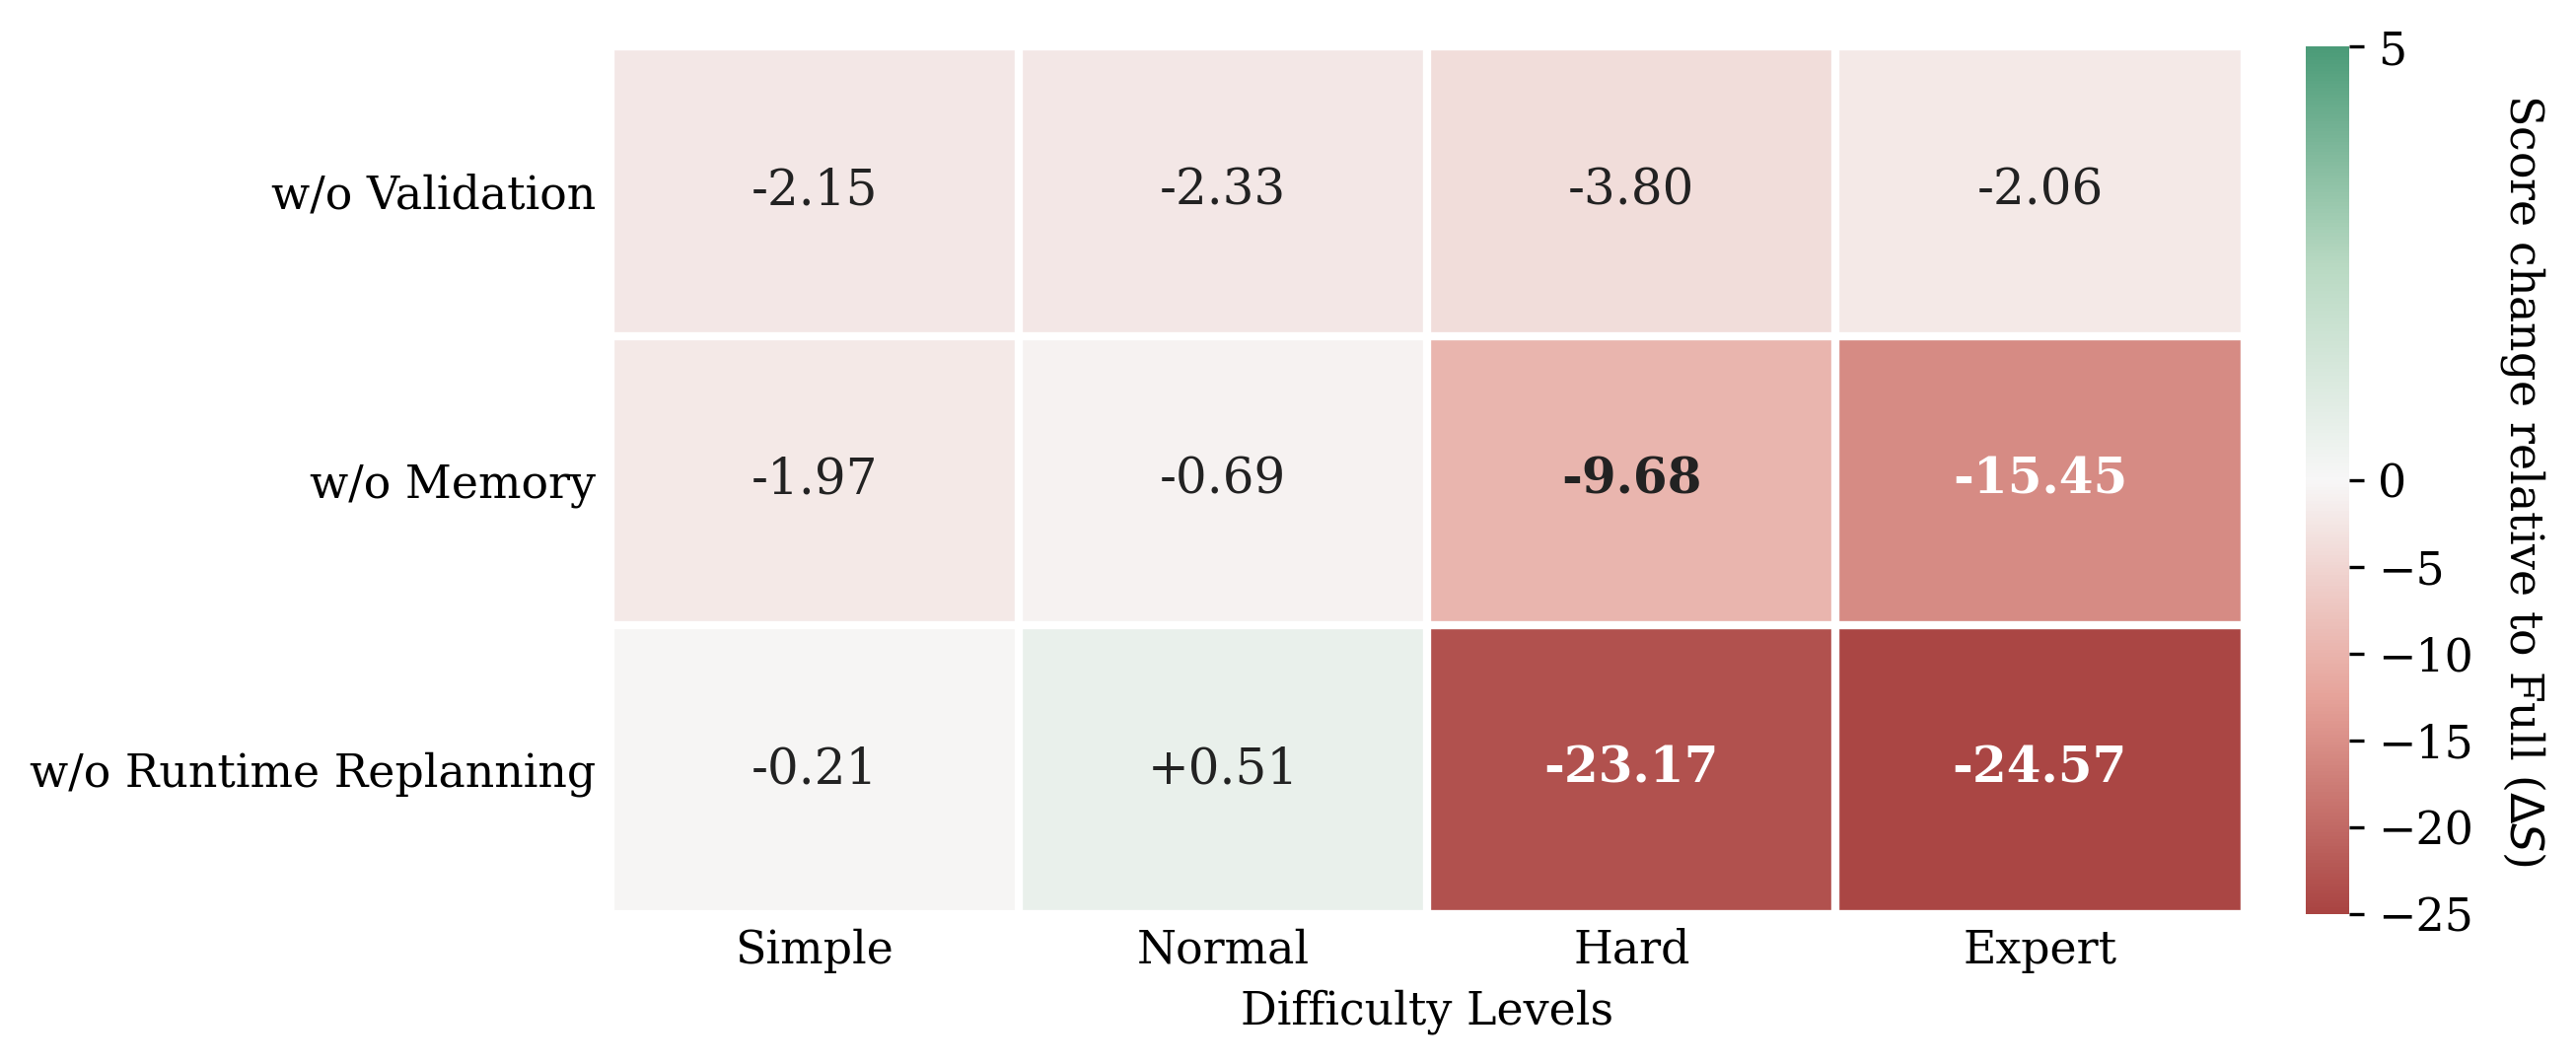
\includegraphics[width=\columnwidth]{figures/ablation-score-change-heatmap.png}
    \caption{Change in overall score relative to the full system for each
    ablated variant and difficulty level. Negative values indicate performance
    degradation, while positive values indicate improvement.}
    \label{fig:ablation-score-delta}
\end{figure}

The contribution of Memory becomes more pronounced as operational pressure
increases.
Removing both memory modules reduces the score by only 1.97 points in the
simple setting and 0.69 points in the normal setting, but the reduction grows
to 9.68 points in hard episodes and 15.45 points in expert episodes. This
pattern indicates that retrieved cases and distilled lessons are most useful
when resource constraints, event interactions, and scheduling pressure make
planning less routine.

Disabling Runtime Replanning has little effect in the simple and normal
settings, where no perturbations are triggered. In contrast, its score falls
from 59.03 to 35.86 in hard episodes and from 37.55 to 12.98 in expert
episodes. The sharp degradation confirms that an initially valid plan is
insufficient once the execution state changes, and that Runtime Replanning is
the key mechanism for maintaining mission performance under perturbations.

The ablations therefore do not indicate three mechanisms that contribute
uniformly in every episode. Validation acts as a low-frequency safeguard
against invalid candidate plans, Memory contributes most when operational
pressure makes planning less routine, and Runtime Replanning becomes critical
when runtime perturbations invalidate an accepted plan. Their condition-dependent
effects explain why all three are retained in the closed-loop framework despite
their different average score contributions.

\subsection{Fine-Tuned Planner Evaluation}

The final experiment concerns deployment of Mission Planning. It asks whether
validated demonstrations can specialize a compact planner for the simple and
normal conditions in which Runtime Replanning is not invoked.

\begin{figure}[!t]
    \centering
    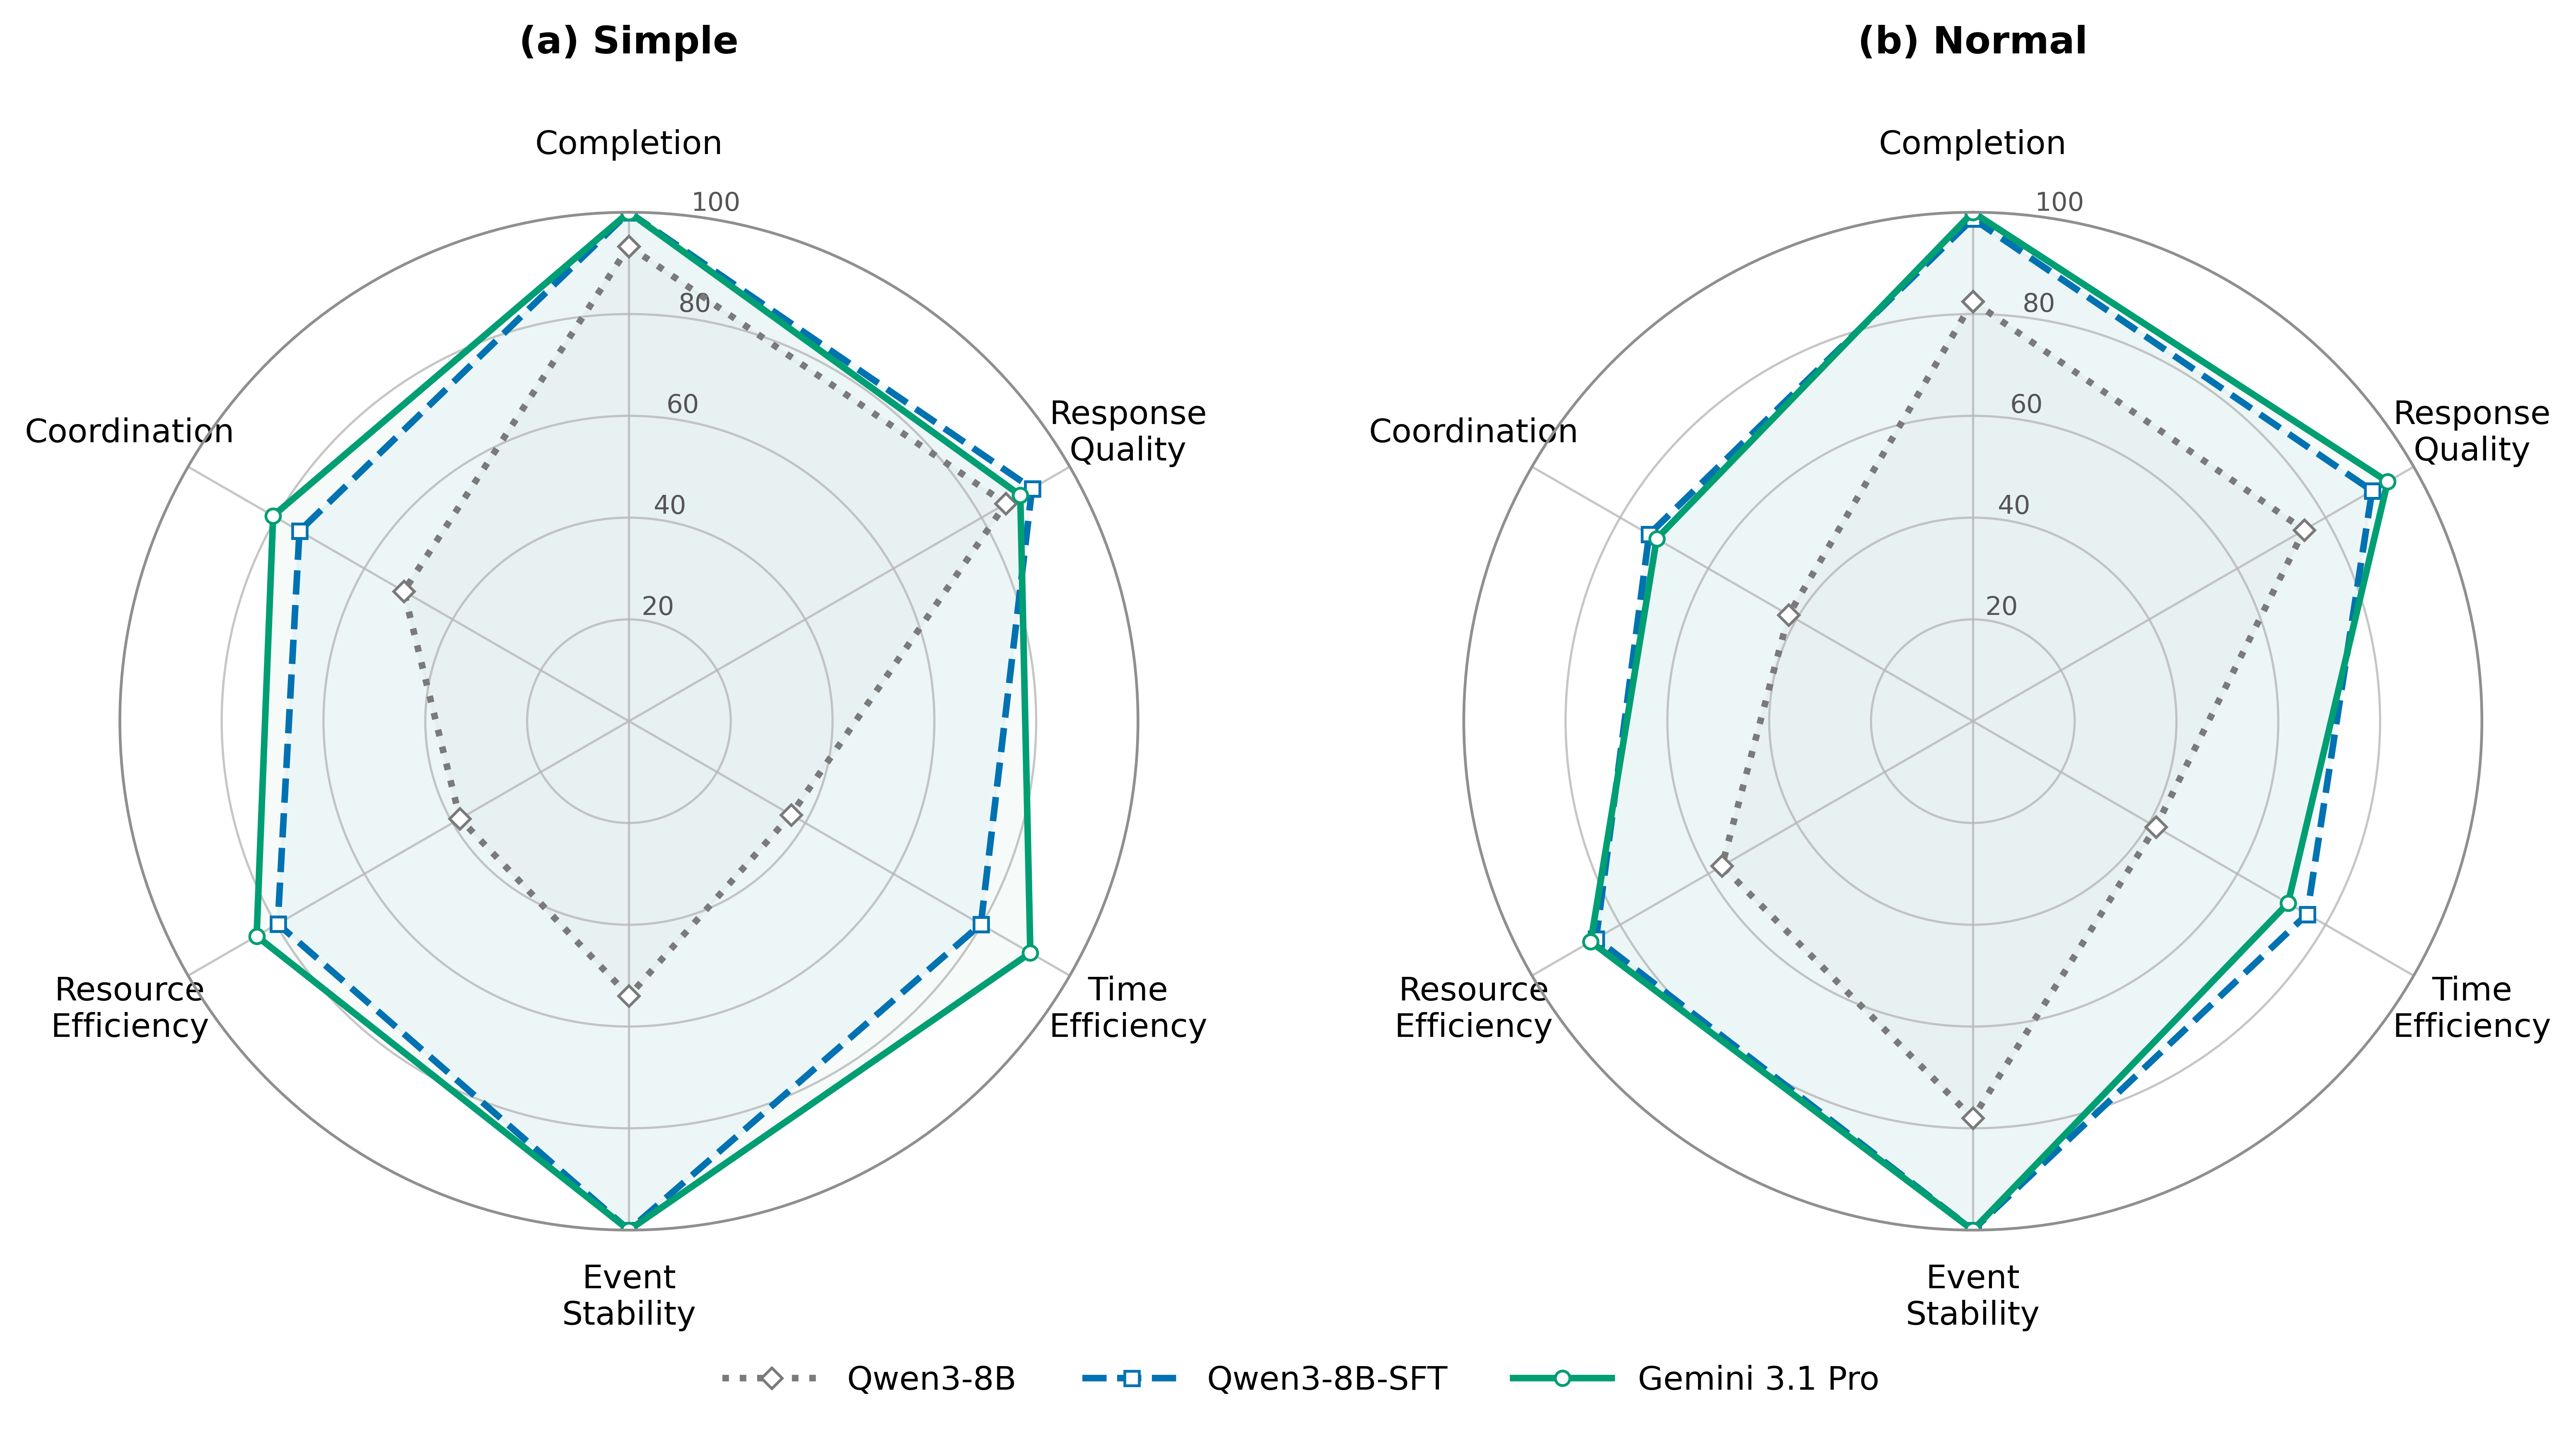
\includegraphics[width=\columnwidth]{figures/planner-performance-radar.png}
    \caption{Mission-level profiles of the three planners in the simple and
    normal settings. Larger radial values indicate better performance. Event
    stability is not interpreted because neither setting contains runtime
    perturbations.}
    \label{fig:planner-performance-radar}
\end{figure}

\begin{figure*}[!b]
    \centering
    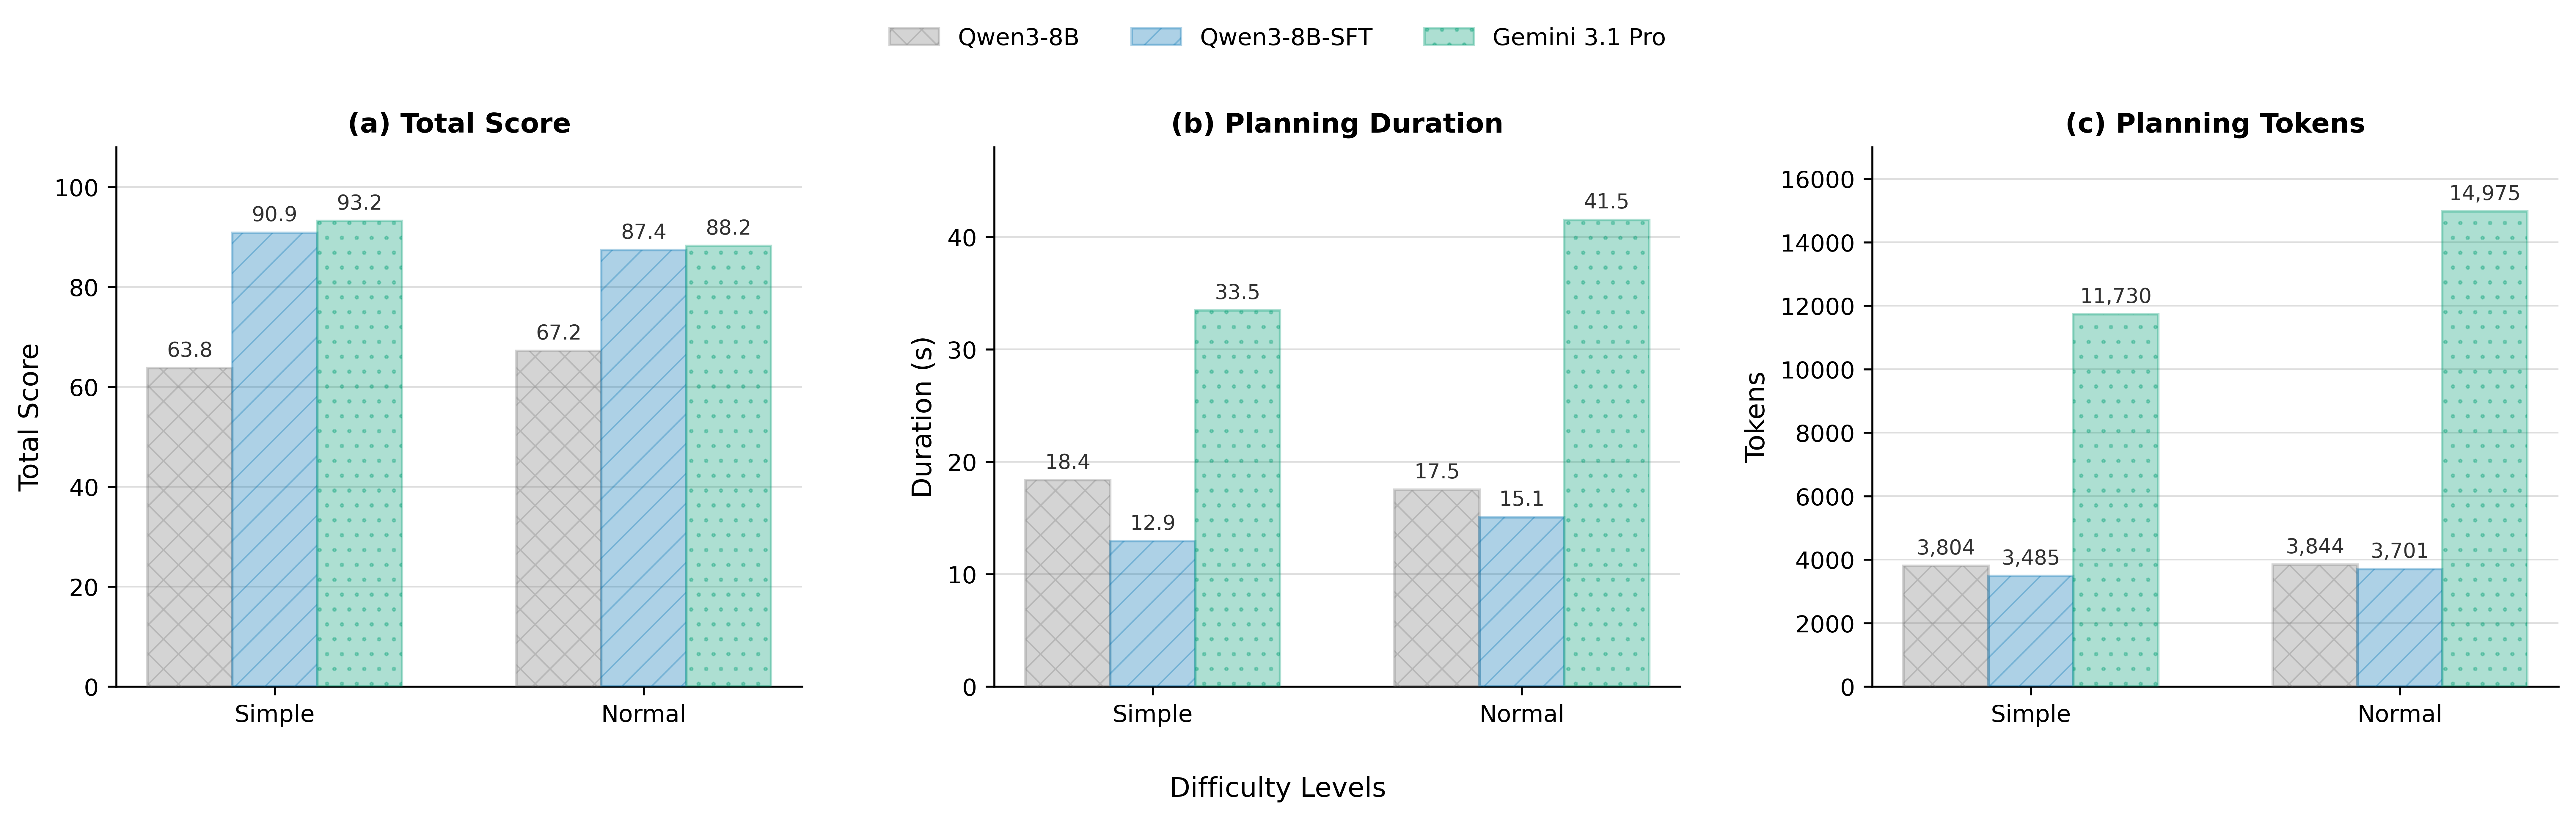
\includegraphics[width=\textwidth]{figures/planner-score-efficiency-comparison.png}
    \caption{Score--efficiency comparison of the three planners: (a) total
    score, (b) planning duration, and (c) planning-token usage. Lower values are
    better in (b) and (c).}
    \label{fig:planner-score-efficiency}
\end{figure*}

Table~\ref{tab:fine-tuned-planner-results} compares the Gemini~3.1~Pro
teacher planner with the original and fine-tuned Qwen3-8B planners. Fine-tuning
substantially improves the compact planner on both difficulty levels. The
overall score increases from 63.77 to 90.87 in the simple setting and from 67.19 to
87.39 in the normal setting. Averaged over the two levels, fine-tuning yields
an absolute gain of 23.65 points and raises Qwen3-8B to 98.24\% of the
Gemini~3.1~Pro teacher planner's average score.

\input{tables/planner-fine-tuning-results}

Figure~\ref{fig:planner-performance-radar} shows that the improvement extends
across the mission-level performance profile. The original Qwen3-8B exhibits
its largest deficits in mission time, resource pressure, and coordination,
whereas fine-tuning substantially expands its profile toward that of
Gemini~3.1~Pro. The fine-tuned planner restores near-complete task coverage and
slightly exceeds Gemini~3.1~Pro in simple-level response and normal-level
mission time and coordination. This indicates that the validated demonstrations
transfer not only output-format compliance but also task-allocation and
resource-management behavior to the compact planner.

The fine-tuned planner also reduces planning overhead under the evaluated
deployment setting. Its mean planning time across the two levels is 14.01~s,
compared with 37.50~s for Gemini~3.1~Pro, while its mean planning-token usage
falls from 13,353 to 3,593. At the individual difficulty levels, this
corresponds to planning-time reductions of 61.3\% and 63.7\%, and token
reductions of 70.3\% and 75.3\%, for simple and normal episodes,
respectively. Figure~\ref{fig:planner-score-efficiency} summarizes this
performance--efficiency trade-off: fine-tuning closes most of the score gap to
the teacher while reducing both planning latency and token usage. These results
show that domain specialization enables Qwen3-8B to retain most of the teacher
planner's mission performance while providing a more efficient locally
deployable alternative for resource-constrained mission planning. This evidence
is limited to initial planning on the evaluated simple and normal episodes; it
does not establish how the compact planner would perform with Runtime
Replanning under hard or expert conditions.

\FloatBarrier

\endinput
